\documentclass[12pt,a4paper]{article}

% Pacotes essenciais
\usepackage{karnaugh-map}
\usepackage[utf8]{inputenc}
\usepackage[T1]{fontenc}
\usepackage[portuguese]{babel}
\usepackage{indentfirst}
\usepackage{amsmath, amsfonts, amssymb}
\usepackage{graphicx}
\usepackage{booktabs}
\usepackage{multirow}
\usepackage{float}
\usepackage{geometry}
\geometry{top=3cm, bottom=2cm, left=3cm, right=2cm}
\setlength{\parindent}{1.25cm}
\usepackage{hyperref}

\graphicspath{{imagens/}}

\title{\textbf{Laborat\'orio EEA-21 -- 3\textordfeminine\ Experi\^encia}\\ \large Projeto e Montagem de Redes Iterativas}
\author{Equipe: Marcello Ryaj e Mateus Levi/ Turma: Comp 28}
\date{\today}

\begin{document}

\maketitle
\tableofcontents
\newpage

% ---------------------------------------------------------
\section{Tarefa 5.1: Montagem de um circuito combinacional com portas NAND2}


A Porta XOR foi construída seguindo o esquemático realizado pelo professor, ao término da montagem, foi testado todas as 4 combinações de entradas possíveis, chegando a seguinte tabela verdade

\begin{table}[H]
    \centering
    \caption{Tabela-verdade obtida para a saída da porta lógica XOR construída}
    \begin{tabular}{ccc}
        \toprule
        $A$ & $B$ & $F$ \\
        \midrule
        0   & 0   & 0   \\
        0   & 1   & 1   \\
        1   & 0   & 1   \\
        1   & 1   & 0   \\
        \bottomrule
    \end{tabular}
    \label{tab:tableXor}
\end{table}

A partir da tabela verdade construída, vemos que a saída F bate com o resultado esperado para uma porta XOR de duas entradas, dessa maneira:

\begin{equation}
    F = A \oplus B
\end{equation}

% ---------------------------------------------------------
\section{Tarefa 5.2: Projeto e montagem da celula basica de um comparador}

Foi solicitado o projeto da celula basica de um comparador iterativo de duas palavras de $n$ bits. As saidas devem indicar, a cada etapa, se a palavra $A$ e maior que $B$, igual a $B$ ou menor que $B$. O relatorio deve apresentar a tabela-verdade da celula, as funcoes logicas obtidas, a montagem em protoboard e a descricao do funcionamento da rede iterativa.

\subsection{Tabela-verdade da celula}

\begin{table}[H]
    \centering
    \caption{Tabela-verdade da celula basica do comparador.}
    \begin{tabular}{ccccccc}
        \toprule
        $A_i$ & $B_i$ & $Y_{1,i}$ & $Y_{3,i}$ & $Y_{1,i-1}$ & $Y_{2,i-1}$ & $Y_{3,i-1}$ \\
        \midrule
        0 & 0 & 0 & 0 & & & \\
        0 & 0 & 0 & 1 & & & \\
        0 & 1 & 0 & 0 & & & \\
        0 & 1 & 0 & 1 & & & \\
        1 & 0 & 0 & 0 & & & \\
        1 & 0 & 0 & 1 & & & \\
        1 & 1 & 0 & 0 & & & \\
        1 & 1 & 0 & 1 & & & \\
        \bottomrule
    \end{tabular}
\end{table}

\subsection{Funcoes logicas}

\[
Y_{1,i-1} = \underline{\hspace{8cm}}
\]

\[
Y_{2,i-1} = \underline{\hspace{8cm}}
\]

\[
Y_{3,i-1} = \underline{\hspace{8cm}}
\]

\subsection{Montagem}

\begin{figure}[H]
    \centering
    % \includegraphics[width=0.8\textwidth]{questao2/comparador_1bit.png}
    \fbox{\rule{0pt}{5cm}\rule{0.8\textwidth}{0pt}}
    \caption{Espaco reservado para a montagem da celula do comparador.}
\end{figure}

\subsection{Resultados experimentais}

\begin{table}[H]
    \centering
    \caption{Resultados obtidos para a celula basica do comparador.}
    \begin{tabular}{ccccccc}
        \toprule
        $A_i$ & $B_i$ & $Y_{1,i}$ & $Y_{3,i}$ & $Y_{1,i-1}$ & $Y_{2,i-1}$ & $Y_{3,i-1}$ \\
        \midrule
        & & & & & & \\
        & & & & & & \\
        & & & & & & \\
        & & & & & & \\
        \bottomrule
    \end{tabular}
\end{table}

\subsection{Rede iterativa}

Explique aqui como as celulas sao encadeadas para formar um comparador de $n$ bits e como se obtem as saidas globais $Y_1$, $Y_2$ e $Y_3$.


% ---------------------------------------------------------
\section{Tarefa 5.3: Projeto e montagem de um subtrator completo de 1 bit}

Nesta etapa, foi solicitado projetar e montar um subtrator completo de 1 bit com propagacao do empresta-um. A celula basica deve produzir a diferenca $S_i$ e o sinal de emprestimo $E_{i-1}$ a partir das entradas $A_i$, $B_i$ e $E_i$, utilizando somente portas NAND de duas entradas na implementacao final.

\subsection{Tabela-verdade}

\begin{table}[H]
    \centering
    \caption{Tabela-verdade da celula do subtrator completo.}
    \begin{tabular}{ccccc}
        \toprule
        $A_i$ & $B_i$ & $E_i$ & $S_i$ & $E_{i-1}$ \\
        \midrule
        0 & 0 & 0 & & \\
        0 & 0 & 1 & & \\
        0 & 1 & 0 & & \\
        0 & 1 & 1 & & \\
        1 & 0 & 0 & & \\
        1 & 0 & 1 & & \\
        1 & 1 & 0 & & \\
        1 & 1 & 1 & & \\
        \bottomrule
    \end{tabular}
\end{table}

\subsection{Expressoes logicas}

\[
S_i = \underline{\hspace{8cm}}
\]

\[
E_{i-1} = \underline{\hspace{8cm}}
\]

\subsection{Implementacao usando NAND2}

Mostre aqui a minimizacao das expressoes e a reescrita em uma forma adequada para implementacao apenas com portas NAND de duas entradas. Se desejar, inclua mapas de Karnaugh ou transformacoes algebricas.

\begin{figure}[H]
    \centering
    % \includegraphics[width=0.8\textwidth]{questao3/subtrator_nand.png}
    \fbox{\rule{0pt}{5cm}\rule{0.8\textwidth}{0pt}}
    \caption{Espaco reservado para o circuito em NAND2 do subtrator completo.}
\end{figure}

\subsection{Resultados experimentais}

\begin{table}[H]
    \centering
    \caption{Resultados experimentais do subtrator completo de 1 bit.}
    \begin{tabular}{ccccc}
        \toprule
        $A_i$ & $B_i$ & $E_i$ & $S_i$ & $E_{i-1}$ \\
        \midrule
        0 & 0 & 0 & & \\
        0 & 0 & 1 & & \\
        0 & 1 & 0 & & \\
        0 & 1 & 1 & & \\
        1 & 0 & 0 & & \\
        1 & 0 & 1 & & \\
        1 & 1 & 0 & & \\
        1 & 1 & 1 & & \\
        \bottomrule
    \end{tabular}
\end{table}

Compare aqui os resultados medidos com os valores esperados teoricamente.


% ---------------------------------------------------------
\section{Tarefa 5.4: Projeto e montagem de um somador completo de 1 bit}

Esta tarefa consistiu no projeto de um somador completo de 1 bit com propagacao do vai-um. A celula basica deve produzir a soma $S_i$ e o transporte $C_{i-1}$ a partir das entradas $A_i$, $B_i$ e $C_i$, com implementacao final usando somente portas NAND de duas entradas.

\subsection{Tabela-verdade}

\begin{table}[H]
    \centering
    \caption{Tabela-verdade da celula do somador completo.}
    \begin{tabular}{ccccc}
        \toprule
        $A_i$ & $B_i$ & $C_i$ & $S_i$ & $C_{i-1}$ \\
        \midrule
        0 & 0 & 0 & & \\
        0 & 0 & 1 & & \\
        0 & 1 & 0 & & \\
        0 & 1 & 1 & & \\
        1 & 0 & 0 & & \\
        1 & 0 & 1 & & \\
        1 & 1 & 0 & & \\
        1 & 1 & 1 & & \\
        \bottomrule
    \end{tabular}
\end{table}

\subsection{Expressoes logicas}

\[
S_i = \underline{\hspace{8cm}}
\]

\[
C_{i-1} = \underline{\hspace{8cm}}
\]

\subsection{Implementacao usando NAND2}

Apresente aqui a minimizacao das expressoes e a implementacao usando somente portas NAND de duas entradas.

\begin{figure}[H]
    \centering
    % \includegraphics[width=0.8\textwidth]{questao4/somador_nand.png}
    \fbox{\rule{0pt}{5cm}\rule{0.8\textwidth}{0pt}}
    \caption{Espaco reservado para o circuito em NAND2 do somador completo.}
\end{figure}

\subsection{Resultados experimentais}

\begin{table}[H]
    \centering
    \caption{Resultados experimentais do somador completo de 1 bit.}
    \begin{tabular}{ccccc}
        \toprule
        $A_i$ & $B_i$ & $C_i$ & $S_i$ & $C_{i-1}$ \\
        \midrule
        0 & 0 & 0 & & \\
        0 & 0 & 1 & & \\
        0 & 1 & 0 & & \\
        0 & 1 & 1 & & \\
        1 & 0 & 0 & & \\
        1 & 0 & 1 & & \\
        1 & 1 & 0 & & \\
        1 & 1 & 1 & & \\
        \bottomrule
    \end{tabular}
\end{table}

Discuta aqui a coerencia entre os resultados observados e o comportamento esperado.


% ---------------------------------------------------------
\section{Tarefa 6.1: Projeto e simula\c{c}\~ao de um circuito multiplicador de 2 bits}

O projeto foi feito a partir da gera\c{c}\~ao dos produtos parciais com portas AND entre os bits de entrada $A_1A_0$ e $B_1B_0$. O bit menos significativo \'e dado diretamente por $C_0 = A_0B_0$. Para o segundo bit, somam-se os termos cruzados $A_0B_1$ e $A_1B_0$ com uma porta XOR, produzindo $M_1$. O terceiro bit \'e obtido com a soma (XOR) entre $A_1B_1$ e o carry da soma anterior, que \'e $(A_0B_1)(A_1B_0)$, resultando em $M_2$. Por fim, o bit mais significativo $M_3$ corresponde ao carry final, implementado no esquem\'atico como o produto $A_1A_0B_1B_0$.

\begin{figure}[H]
    \centering
    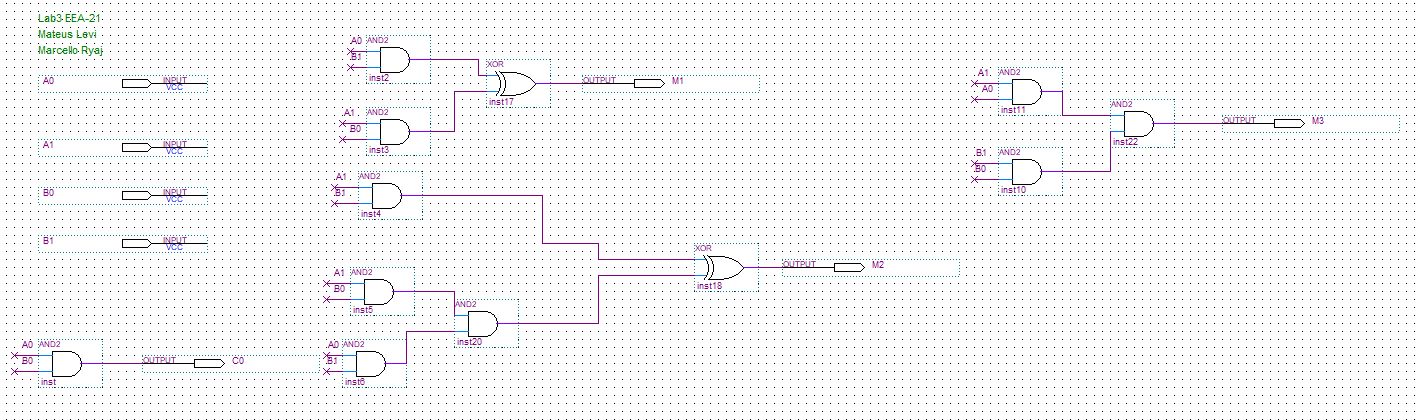
\includegraphics[width=0.95\textwidth]{esquematico.png}
    \caption{Diagrama esquem\'atico do multiplicador de 2 bits.}
\end{figure}

\subsection{Equa\c{c}\~oes do circuito}

\[
    P_0 = C_0 = A_0 \cdot B_0
\]

\[
    P_1 = M_1 = (A_0 \cdot B_1) \oplus (A_1 \cdot B_0)
\]

\[
    P_2 = M_2 = (A_1 \cdot B_1) \oplus \left[(A_0 \cdot B_1) \cdot (A_1 \cdot B_0)\right]
\]

\[
    P_3 = M_3 = A_1 \cdot A_0 \cdot B_1 \cdot B_0
\]

\subsection{Simula\c{c}\~ao funcional}


\begin{figure}[H]
    \centering
    \includegraphics[width=0.9\textwidth]{\detokenize{produto 1011.png}}
    \caption{Temporiza\c{c}\~ao para $(10)_b \times (11)_b$ (entrada 1011, sa\'ida 0110).}
\end{figure}

\begin{figure}[H]
    \centering
    \includegraphics[width=0.9\textwidth]{\detokenize{produto 1000.png}}
    \caption{Temporiza\c{c}\~ao para $(10)_b \times (00)_b$ (entrada 1000, sa\'ida 0000).}
\end{figure}

\begin{figure}[H]
    \centering
    \includegraphics[width=0.9\textwidth]{\detokenize{produto 0101.png}}
    \caption{Temporiza\c{c}\~ao para $(01)_b \times (01)_b$ (entrada 0101, sa\'ida 0001).}
\end{figure}

\begin{figure}[H]
    \centering
    \includegraphics[width=0.9\textwidth]{\detokenize{produto 1111.png}}
    \caption{Temporiza\c{c}\~ao para $(11)_b \times (11)_b$ (entrada 1111, sa\'ida 1001).}
\end{figure}

\begin{table}[H]
    \centering
    \caption{Resultados esperados para os casos simulados.}
    \begin{tabular}{ccc}
        \toprule
        Opera\c{c}\~ao          & Resultado esperado & Resultado simulado \\
        \midrule
        $(10)_b \times (11)_b$ & $(0110)_b$         & $(0110)_b$         \\
        $(10)_b \times (00)_b$ & $(0000)_b$         & $(0000)_b$         \\
        $(01)_b \times (01)_b$ & $(0001)_b$         & $(0001)_b$         \\
        $(11)_b \times (11)_b$ & $(1001)_b$         & $(1001)_b$         \\
        \bottomrule
    \end{tabular}
\end{table}

\subsection{Coment\'arios}

    Os resultados simulados coincidem com os valores esperados para os quatro casos pedidos no roteiro. Isso confirma que o esquem\'atico implementa corretamente a multiplica\c{c}\~ao de 2 bits, com sa\'ida organizada como $P_3P_2P_1P_0 = M_3M_2M_1C_0$.


\end{document}
